\documentclass{article}
\usepackage{graphicx}
% \usepackage{array}
% \usepackage{multirow}
\usepackage{hyperref}
% \usepackage{booktabs}

\begin{document}

\title{Project 2}
\author{Jake Carlson}
\date{October 4, 2017}
\maketitle

\abstract
Classification on federal payroll data.
\newpage

\tableofcontents
\newpage

\section{Business Understanding}
In this project, I will again be analyzing the federal payroll data obtained by BuzzFeed News through the Freedom of Information Act. I will continue my analysis of the presidency of George W. Bush and Barack Obama by creating classification models based on the payroll data. Based on attributes of the employees, I will be trying to predict class labels such as the annual pay of the employee, what their level of education is, how long they have been a federal employee, what their supervisory status is, and where they are located. The various models will provide insight into how relevant each attribute is as predicitng the class label. For example, the heirarchy of splits in decision trees indicate what attributes are most relevant when determining the class label. By looking at how these models differ between the presidents, and how the ranking of attributes changes, we will gain insight into how each administration restructured the composition of the federal government.
\par
I will use a variety of classification models, including Decision Trees, K-Nearest Neighbors, PART, Artificial Neural Networks, and Random Forests. I will compare the performance of these models to each other to see what models have the best performance in terms of both accuracy and the time required to perform classification on test data.

    \subsection{Annual Pay}
    By predicting Pay, we will see what attributes correspond to a higher pay rate. This would be useful for employees so that they can see what attributes they should look to change about themselves if they are looking to get a pay raise. For example, if Education has a strong relationship with higher pay rates, employees should consider pursuing higher education in order to recieve a raise.

    \subsection{Education Level}
    By predicting Education, we will be able to see what attributes are most related with having a higher or lower education level. If a particular agency is in need additional specialized labor, they could offer a subset of their employees financial aid to pursue higher education. This would allow that agency to promote from within, rather than looking for new employees.
    \par
    From Project 1 we determined that the vast majority of employees had either a high school diploma or a Bachelor's degree. This class imbalance will need to be addressed when creating classification models.\cite{proj1}

    \subsection{Length of Service}
    By predicting Length of Service, we will see what factors encourage employees to continue their work at the federal government. By examining how the most imporant attributes change between administrations, we will get an idea of what each administration favored in their employees. We will also see what types of employees prefered to continue their employement in response to the leadership change. Useful why??

    \subsection{Supervisory Status}
    By seeing what factors affect Supervisory Status, we will see what the most common attributes are for members of leadership within an agency. This could be used by each agency to see if their leadership is biased to employees with certian attributes. With this information, agencies could work to diversify their leadership and potentially improve the operations of their agency and improve the propensity of potential employees to apply for employment from that agency. A more diverse applicant pool would allow the agency to restructure more efficiently under new leadership.

    \subsection{Location}
    By modeling where an employee is located based on their attributes, we can see what the demographics are in each state. By breaking up this model by agency, we can get an idea of how the agency is organized at a national level. We may see more supervisors in the Washington D.C. and Maryland area. With this model, an agency could more easily visualize their structure and, if a certain state is struggling to meet operational requirements, allocate additional supervisors from a state with a surplus to the state that is struggling.
    \par
    Because larger states have more federal employees, we will have a class imbalance where large states are over-represented.

\section{Data Preparation}
To prepare my data for classification, I reprocess the raw payroll data. I start by removing columns that I don't plan on using for classification. The attributes I save are given in Table \ref{tab:1}. I then replace unknown values with NA, make Pay a numeric attribute, pull out the encoding for what state the employee works in from Station, and create a column that holds the whole agency name for each employee. I join the four quarters for each of the four years I'm looking at into one data frame, and save this frame to disk.
\par
When I load these data frames, I run some additional preparation to make sure the data is ready for classification and make sure the models will train as efficiently as possible. I create a region column which translates the state encoding in Station to the actual name of the state. I convert Pay to an ordinal variable from a continuous variable by descretizing into six classes. The Pay groups are given in Table \ref{tab:2}. I then convert the ordinal Age variable to a ratio variable by taking the middle of the age range for each occurance The Age translation is given in Table \ref{tab:3}. I break Education up into groups by what level of education the employee achieved. The groups I used are listed in Table \ref{tab:9}. Next I convert the ordinal Length of Service variable to a ratio varible by taking the middle of the time span for each occurance. The translation for LOS is given in Table \ref{tab:4}. My preparation function also allows for a subset of agencies to be choosen from the saved data files. The last step in the preparation function is converting the agencies to a one-hot encoded representation. This creates a new column for each agency which has a 1 in it if the employee works at that agency, and a 0 if the employee does not work at that agency.
\par
The scale and range of all of the attributes in the final data set are given in Table \ref{tab:5}. When I go to create a model based on a subset of my choosen columns, I will throw out any entries that are incomplete. The count of the number of records that are complete, as well as the percentage of records that are complete for each year are given in Table \ref{tab:6}.

    \begin{center}
        \begin{table}
            \centering
            \begin{tabular}{ |c|c|c| }
                \hline
                Attribute & Scale & Description \\
                \hline
                Agency & Categorical & The four character encoding for the agency the employee worked at. \\
                Station & Categorical & The state the employee works in. \\
                Age & Ordinal & The age range of the employee, given in 5 year intervals. \\
                Education & Ordinal & The education level achieved by the employee. \\
                LOS & Ordinal & The number of years the employee has worked in the federal governemnt, given in 5 year intervals. \\
                Category & Categorical & The general type of work the employee does, following the PATCO acronym. \\
                Pay & Ratio & The annual pay the employee receives in U.S. Dollars. \\
                SupervisoryStatus & Categorical & The level of leadership the employee has achieved. \\
                \hline
            \end{tabular}
            \caption{Attributes To Be Used For Classification}
            \label{tab:1}
        \end{table}
    \end{center}

    \begin{center}
        \begin{table}
            \centering
            \begin{tabular}{ |c| }
                \hline
                Pay Ranges \\
                \hline
                $<$30k \\
                30-50k \\
                50-70k \\
                70-90k \\
                90-110k \\
                $>$110k \\
                \hline
            \end{tabular}
            \caption{The Pay Ranges Used To Descretize Pay}
            \label{tab:2}
        \end{table}
    \end{center}

    \begin{center}
        \begin{table}
            \centering
            \begin{tabular}{ |c|c| }
                \hline
                Age Range & Ratio Value \\
                \hline
                15-19 & 17 \\
                20-24 & 22 \\
                25-29 & 27 \\
                30-34 & 32 \\
                35-39 & 37 \\
                40-44 & 42 \\
                45-49 & 47 \\
                50-54 & 52 \\
                55-59 & 57 \\
                60-64 & 62 \\
                65-69 & 67 \\
                70-74 & 72 \\
                75+ & 75 \\
                \hline
            \end{tabular}
            \caption{Original Age Ranges In Years And The Choosen Value For Classification}
            \label{tab:3}
        \end{table}
    \end{center}

    \begin{center}
        \begin{table}
            \centering
            \begin{tabular}{ |c|c|c| }
                \hline
                Group & Education Levels & Description \\
                \hline
                Elm & 0, 1 & Reached or completed elementary school \\
                HS & 3, 4, 5, 6 & Reached or completed high school or an occupational program \\
                Col & 7, 8, 9, 10, 11, 12, 13 & Reached or completed college with a Bachelor's degree \\
                Grad & 14, 15, 16, 17, 18, 19, 20 & Any level of graduate studies, excluding a Doctorate \\
                Doc & 21, 22 & A Doctorate or Post-Doctorate degree \\
                \hline
            \end{tabular}
            \caption{Ordinal Education Groups}
            \label{tab:9}
        \end{table}
    \end{center}

    \begin{center}
        \begin{table}
            \centering
            \begin{tabular}{ |c|c| }
                \hline
                LOS Range & Ratio Value \\
                \hline
                $<$ 1 & 1 \\
                1-2 & 1 \\
                3-4 & 3 \\
                5-9 & 7 \\
                10-14 & 12 \\
                15-19 & 17 \\
                20-24 & 22 \\
                25-29 & 27 \\
                30-34 & 32 \\
                35+ & 35 \\
                \hline
            \end{tabular}
            \caption{Original Length Of Service Ranges And The Choosen Value For Classification}
            \label{tab:4}
        \end{table}
    \end{center}

    \begin{center}
        \begin{table}
            \centering
            \begin{tabular}{ |c|c|c| }
                \hline
                Attribute & Scale & Range \\
                \hline
                Agency & Categorical & Unique four characters for each agency \\
                Station & Categorical & 1-56, some values missing \\
                Age & Ratio & 17-72 by 5, 75 \\
                Education & Categorical & 1-22 \\
                LOS & Ratio & 1, 3, 7-32 by 5, 35 \\
                Category & Categorical & P, A, T, C, O, B \\
                Pay & Ordinal & $<$30k, 30-50k, 50-70k, 70-90k, 90-110k, $>$110k \\
                SupervisoryStatus & Categorical & 2, 4, 5, 6, 7, 8 \\
                \hline
            \end{tabular}
            \caption{Final Data Set Attributes}
            \label{tab:5}
        \end{table}
    \end{center}

    \begin{center}
        \begin{table}
            \centering
            \begin{tabular}{ |c|c|c| }
                \hline
                Year & Number Complete & Percentage of Original \\
                \hline
                2001 & 2,535,278 & 58.09\% \\
                2005 & 2,598,800 & 55.05\% \\
                2009 & 2,862,972 & 55.22\% \\
                2013 & 3,136,697 & 58.91\% \\
                \hline
            \end{tabular}
            \caption{The Number Of Complete Records For Each Year}
            \label{tab:6}
        \end{table}
    \end{center}

\section{Modeling}
Next I will begin creating models for the each of the cases outlined in the Business Understanding. I will create two models for each of the cases and compare their performance using 10-fold cross validation. I will select the model that perfoms the best and train it on the data for each of my choosen years. I will then compare these models to see how their structure changes with the presidency. To make training and evaluation easier, I will create a pipeline to break up the data, train the models, test them, and return the results.

    \subsection{Annual Pay}
    I will be modeling Pay for the Department of Justice. I will compare the performace of decision trees and random forests. In order to speed up the training of my models, I only want to pass in the attributes that are most important for predicting Pay. To determine these attributes I examine the results of both cfs, which uses correlation and cross entropy, and consistency, which uses a consistency measure, to determine variable importance. The most important attributes given by consistency in descending order are Age, Education, Length of Service, Category, and SupervisoryStatus. The most important measures by cfs are Education and Category. I will use Age, Education, and Category for training my models.
    \par
    The accuracy and kappa scores for each of the models is given in Table \ref{tab:7}. These scores aren't great, but the random forests consistently beat out the decision tree. The most important variables given by the random forests are Education and Age followed by whether or not the employee is in a technical role or a clerical role. The decision tree concurs with the random forests that Education is the most important attribute, followed by whether the employee is in a techinical role or not. This indicates that the education is strongly related with how much an employee makes in the Department of Justice.
    \par
    The structure of the decision tree given in Figure \ref{paydesctree2005} shows that clerical roles tend to be paid less and technical roles tend to be paid more. I want to see how these models change under the Obama administration, so I will rerun these using the 2013 data set. Again, Education is the most important attribute for both the decision tree and the random forest, followed by Age. The structure of the decision tree for 2013 is given in Figure \ref{paydesctree2013}. We see that the splits in the decision tree closest to the root have to do with what Category an employee is in. The difference in the complexity of the decision tree would appear to indicate that, under the Obama administration, pay was more closely related to what type of position you held.

    \begin{center}
        \begin{table}
            \centering
            \begin{tabular}{ |c|c|c|c|c|c|c|c| }
                \hline
                Accuracy \\
                \hline
                Classifier & Min. & 1st Qu. & Median & Mean & 3rd Qu. & Max. & NA's \\
                Decision Trees & 0.5176392 & 0.5211121 & 0.5275774 & 0.5289369 & 0.5376409 & 0.5415454 & 0 \\
                Random Forests & 0.5619261 & 0.5658214 & 0.5704048 & 0.5698463 & 0.5739125 & 0.5764363 & 0 \\
                \hline
                Kappa \\
                \hline
                Classifier & Min. & 1st Qu. & Median & Mean & 3rd Qu. & Max. & NA's \\
                Decision Trees & 0.3466076 & 0.3497777 & 0.3672808 & 0.3688381 & 0.3881202 & 0.3946472 & 0 \\
                Random Forests & 0.4274982 & 0.4319667 & 0.4382973 & 0.4374711 & 0.4428353 & 0.4456237 & 0 \\
                \hline
            \end{tabular}
            \caption{The Accuracy And Kappa Score for Decision Trees and Random Forests}
            \label{tab:7}
        \end{table}
    \end{center}

    \begin{center}
        \begin{table}
            \centering
            \begin{tabular}{ |c|c|c|c|c| }
                \hline
                % & \multicomlum{2}{|c|}{2005} & \multicomlum{2}{|c|}{2013} \\
                & 2005 & 2005 & 2013 & 2013 \\
                \hline
                Decision Tree & Education & 9932.9 & Education & 9382.2 \\
                & CategoryT & 7682.5 & Age & 7867.3 \\
                & CategoryP & 5599.9 & CategoryP & 5382.3 \\
                & CategotyC & 5305.0 & CategoryB & 4715.5 \\
                \hline
                Random Forest & Education & 10345.0 & Education & 11113.4 \\
                & Age & 4089.5 & Age & 5470.7 \\
                & CategoryT & 2805.7 & CategoryC & 1601.5 \\
                & CategoryC & 2393.5 & CategoryT & 1476.4 \\
                \hline
            \end{tabular}
            \caption{Variable Importance Rankings for Predicting Pay for Decision Trees and Random Forests in 2005 and 2013}
            \label{tab:8}
        \end{table}
    \end{center}

    \begin{center}
        \begin{figure}
            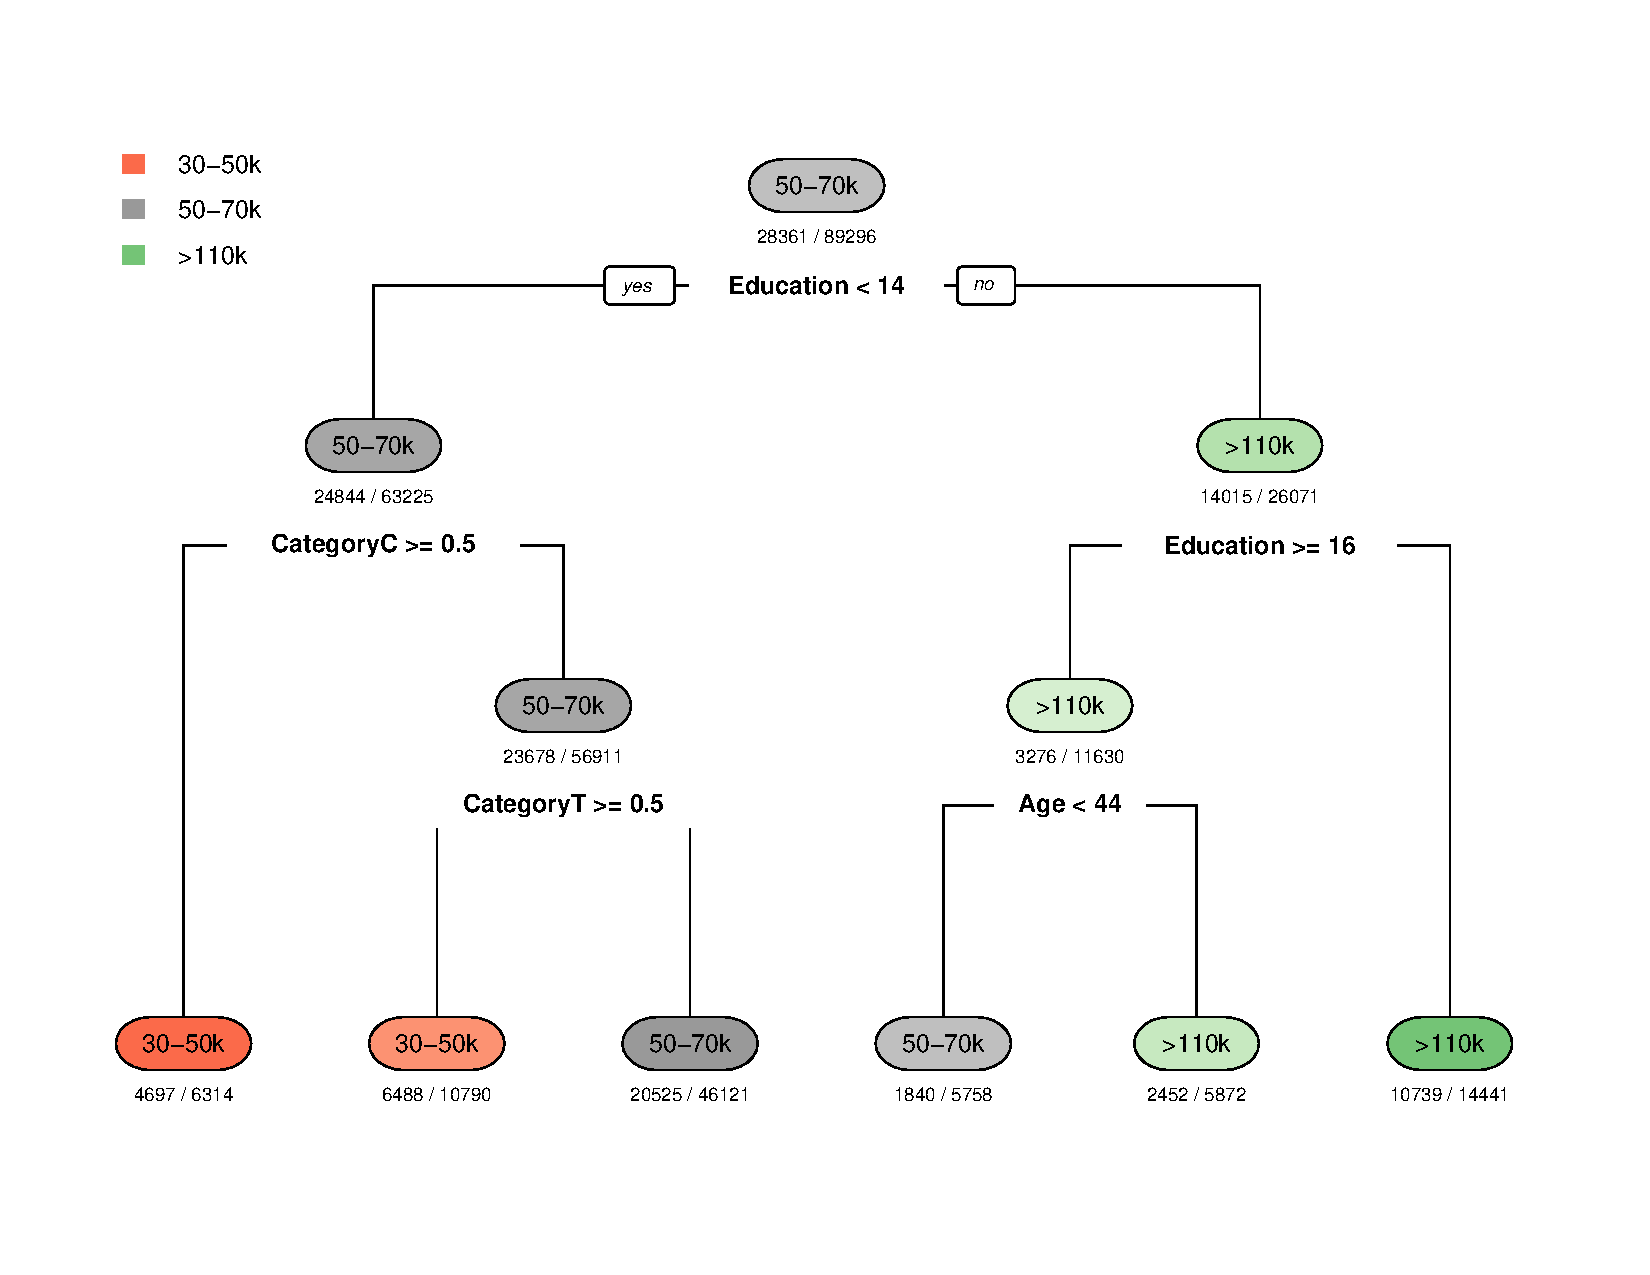
\includegraphics[scale=0.4]{./images/pay-decision-tree-2005.pdf}
            \caption{The Structue of the Decision Tree for Pay in the Department of Justice in 2005}
            \label{paydesctree2005}
        \end{figure}
    \end{center}

    \begin{center}
        \begin{figure}
            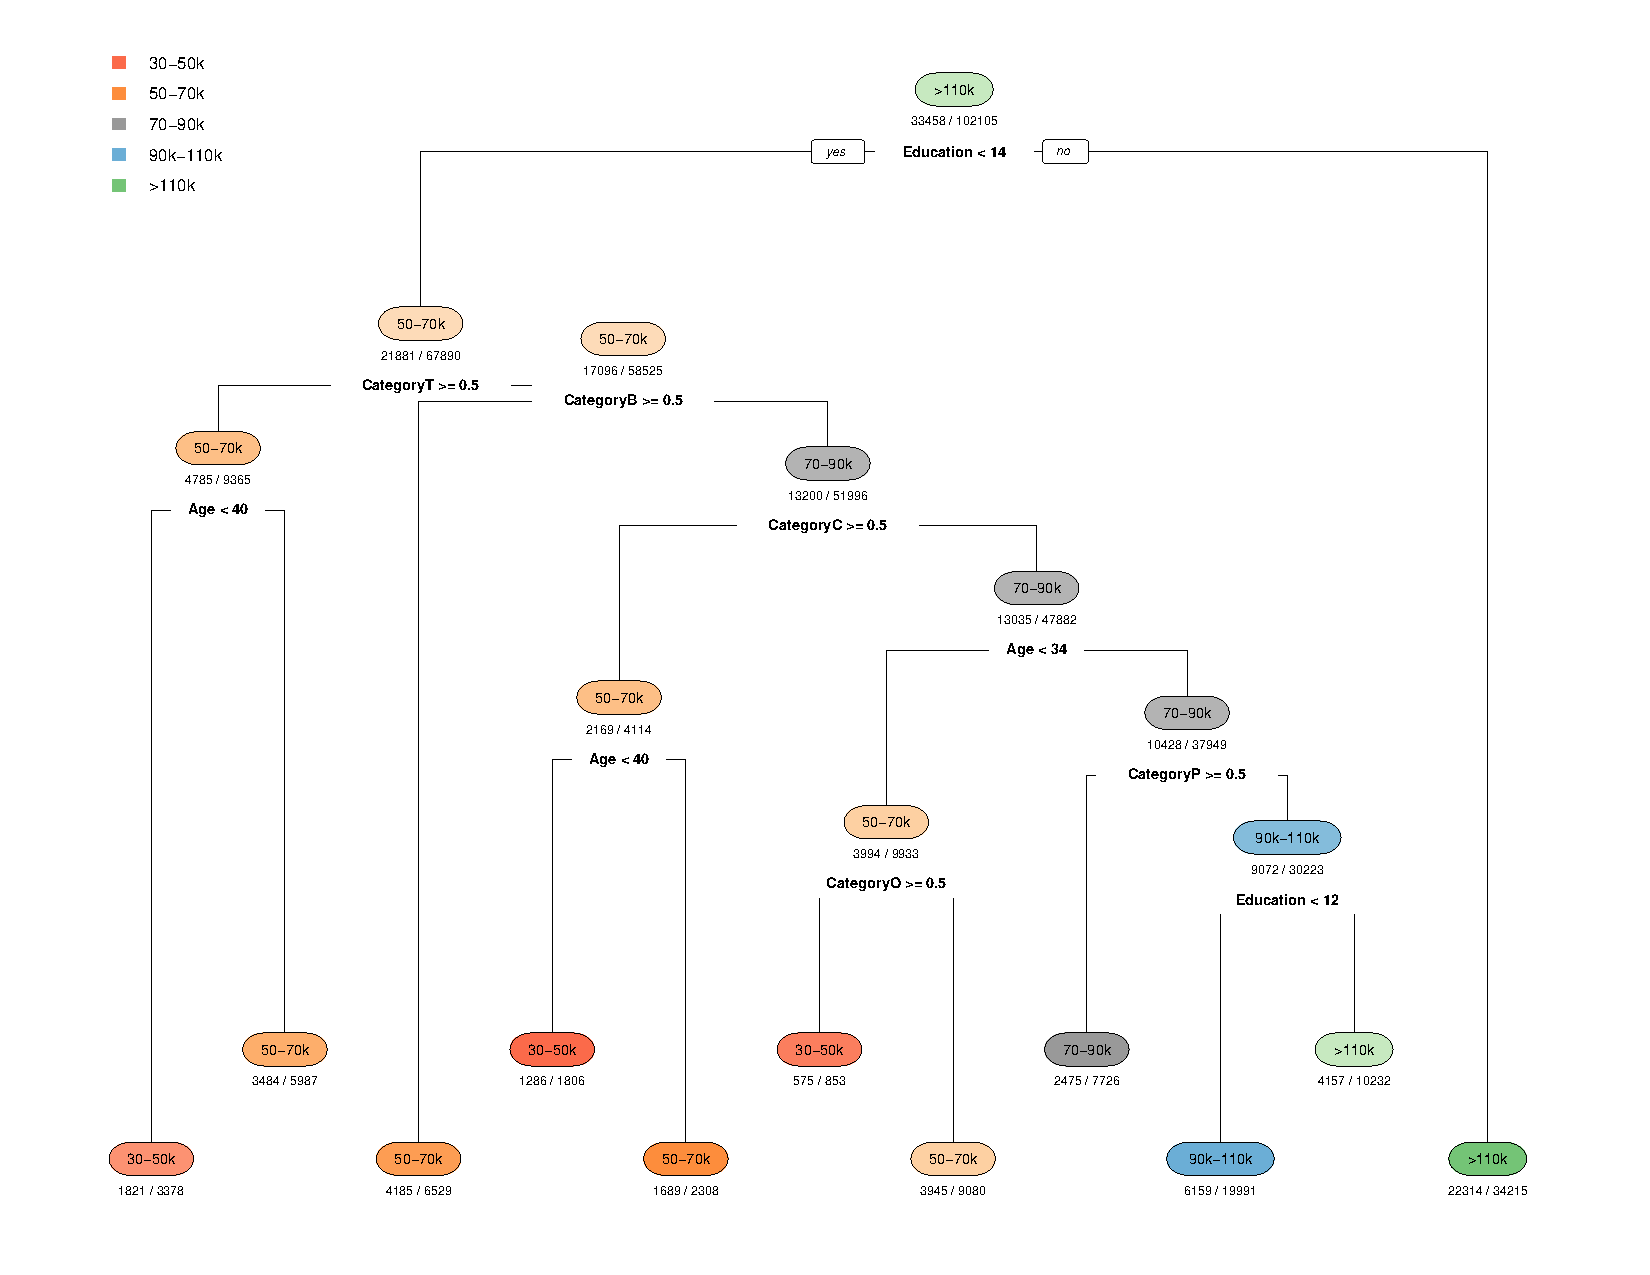
\includegraphics[scale=0.4]{./images/pay-decision-tree-2013.pdf}
            \caption{The Structue of the Decision Tree for Pay in the Department of Justice in 2013}
            \label{paydesctree2013}
        \end{figure}
    \end{center}

    \subsection{Education Level}
    I will model Education for the Department of Justice. The models for Pay showed that the Category and Education are the most relevant attributes for predicting the Pay of an employee. I would expect Category to be an important attribute in predicting Education. I will again use cfs and consistency to determine the most relevant attributes to use when training my models for Education. For this attribute, I will again compare random forests to decision trees. Consistency gives the most important attributes as Age, Length of Service, Category, and SupervisoryStatus. Cfs gives the most important attributes as Category, and Pay. I will use Age, Category, and Pay to build my models. It is important to note that neither of the years I have choosen have employees who reached Doctorate level studies.
    \par
    The models had comparable accuracy and kappa scores to the scores in Table \ref{tab:7}. Again, the random forest consistently beat the decision tree with a maximum accuracy of 0.616 over 0.604 and a maximum kappa of 0.415 over 0.399. The most important attributes for 2005 and 2013 are given in Table \ref{tab:10}. I've also provided the decision tree structure for 2005 in Figure \ref{edudesctree2005} and 2013 in Figure \ref{edudesctree2013}.
    \par
    It is interesting how similar the structures of the trees are. The trees are identical except for the last split between college and graduate education levels. The relationship between reaching graduate studies and having a pay greater than 100k. The most accurate class in both decision trees is where the employee reached graduate level studies and has an annual income greater than 100k. The accuracy of this class actually drops moving from Bush to Obama, indicating employees with lower levels of education were able to reach a higher pay grade.

    \begin{center}
        \begin{table}
            \centering
            \begin{tabular}{ |c|c|c|c|c| }
                \hline
                & 2005 & 2005 & 2013 & 2013 \\
                \hline
                Decision Tree & Pay.110k & 11733.8 & Pay.110k & 11483.9 \\
                & CategoryP & 9518.1 & CategoryP & 10257.4 \\
                & Pay30.50k & 3680.3 & Pay50.70k & 5405.1 \\
                & CategoryB & 2814.5 & CategoryB & 3793.9 \\
                \hline
                Random Forest & CategoryP & 9515.0 & CategoryP & 10257.5 \\
                & Pay.110k & 3171.8 & Pay.110k & 3554.9 \\
                & Age & 930.5 & CategoryB & 1421.8 \\
                & CategoryB & 915.6 & Age & 1384.9 \\
                \hline
            \end{tabular}
            \caption{Variable Importance Rankings for Predicting Education for Decision Trees and Random Forests in 2005 and 2013}
            \label{tab:10}
        \end{table}
    \end{center}

    \begin{center}
        \begin{figure}
            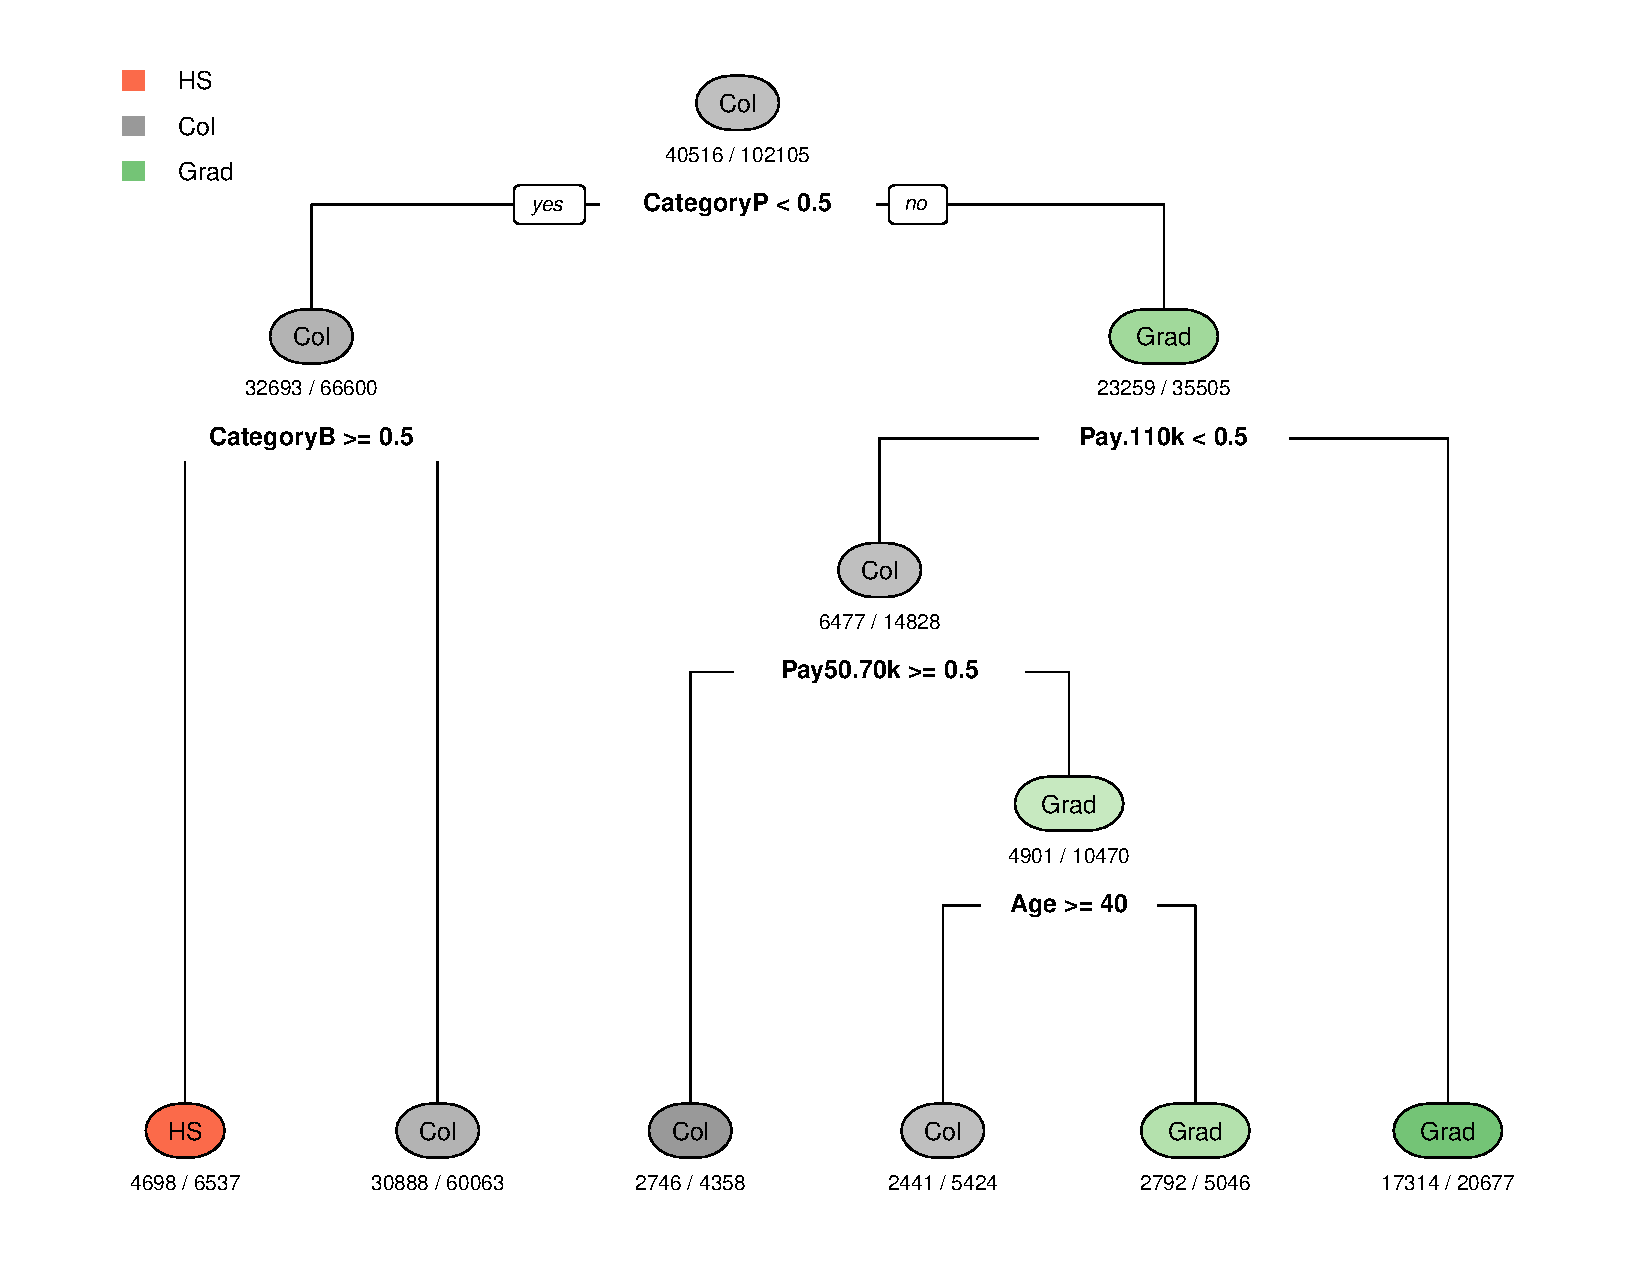
\includegraphics[scale=0.4]{./images/edu-decision-tree-2013.pdf}
            \caption{The Structue of the Decision Tree for Education in the Department of Justice in 2013}
            \label{edudesctree2013}
        \end{figure}
    \end{center}

    \begin{center}
        \begin{figure}
            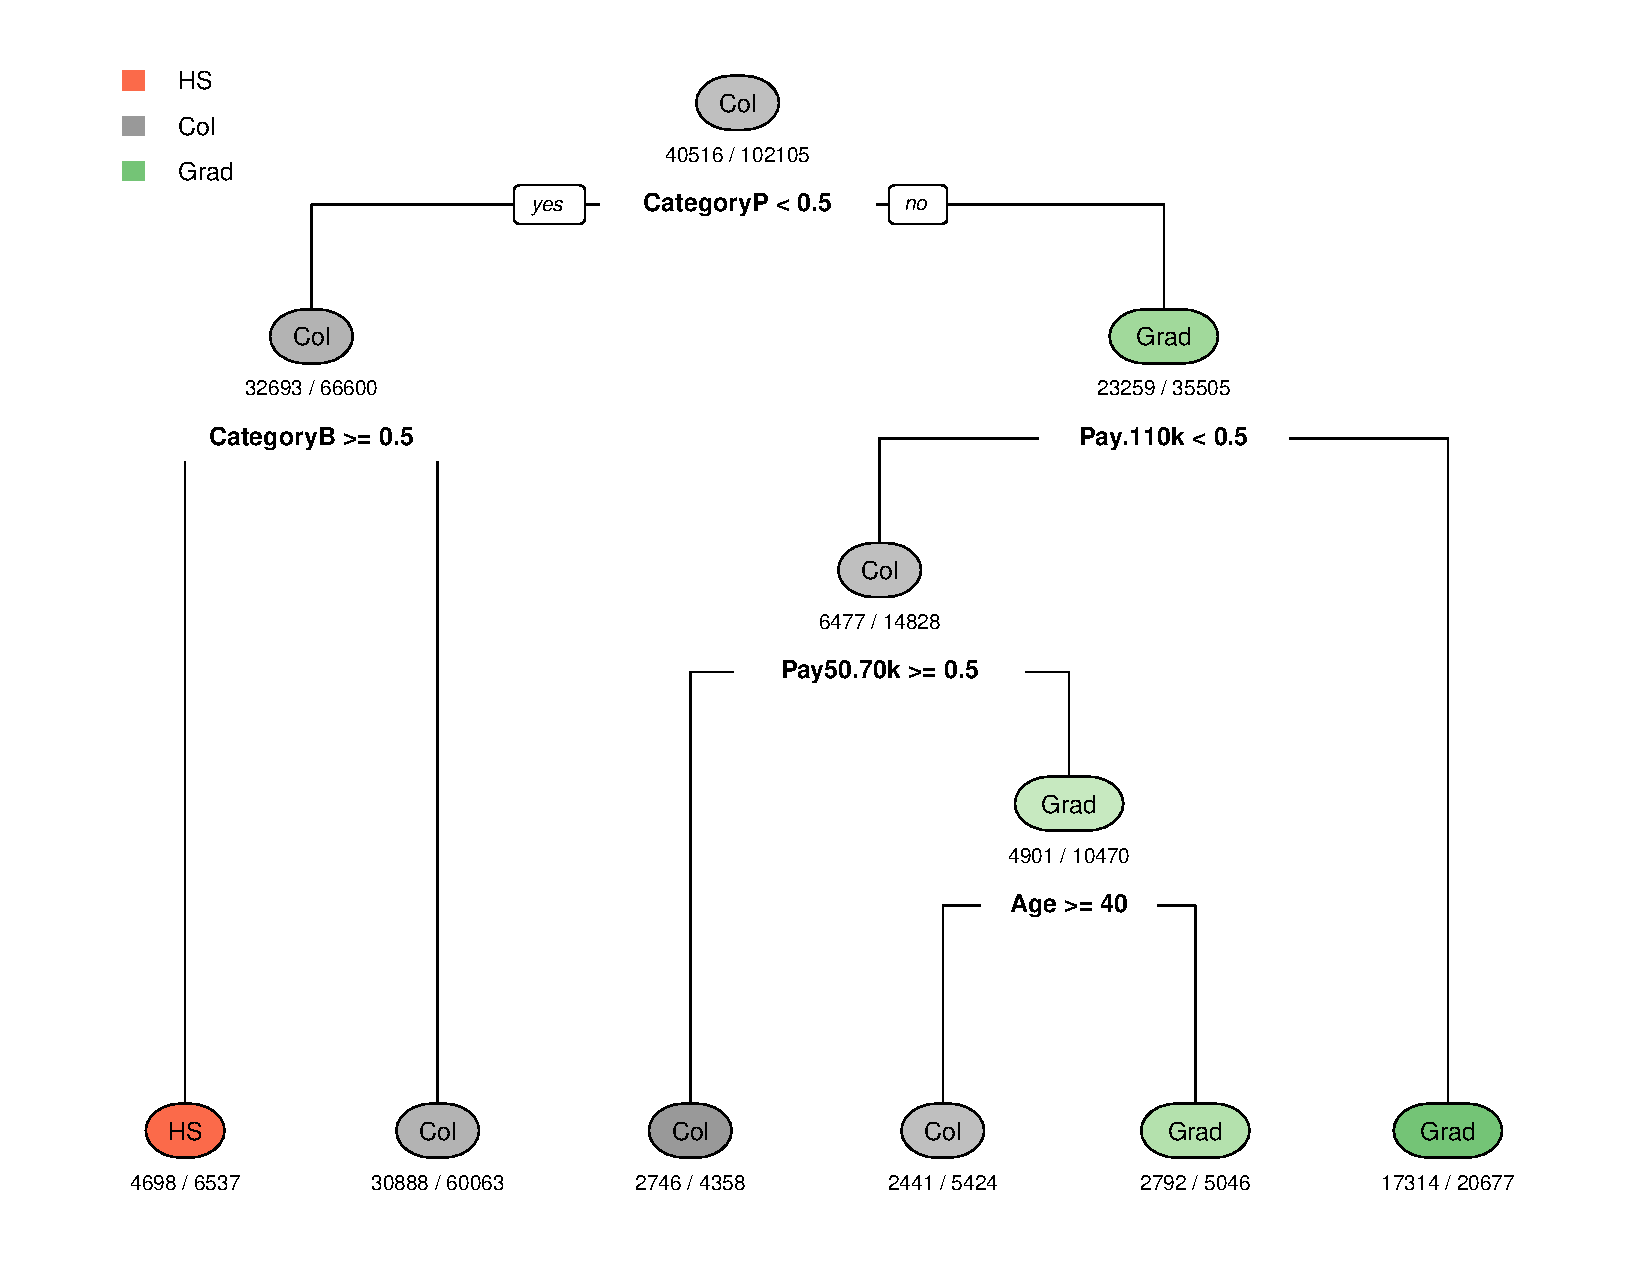
\includegraphics[scale=0.4]{./images/edu-decision-tree-2013.pdf}
            \caption{The Structue of the Decision Tree for Education in the Department of Justice in 2013}
            \label{edudesctree2013}
        \end{figure}
    \end{center}

    \subsection{Length of Service}

    \subsection{Supervisory Status}

    \subsection{Location}

What are the differences across time and between agencies?

\section{Evaluation and Deployment}
Are these models useful for solving the problems outlined in the business understanding?

\begin{thebibliography}{10}
    \bibitem{proj1}
    Jake Carlson
    \textit{CSE 5331 - Data Mining Project 1}
    \texttt{https://github.com/jakecarlson1/data-mining-projects/blob/master/}
    \texttt{project-1/report/carlson-project-1.pdf}

\end{thebibliography}

\end{document}
